\section{Higher alignment interventionally achieves better model performance }

\textbf{Experiment:} We validate compression as an alignment metric by evaluating the impact of a model fine-tuned on more \texttt{ZIP-FIT}-aligned data with a target task and the corresponding cross-entropy (CE) loss.  
We chose ProofNet (test) as the target benchmark and then fine-tuned GPT-2 \cite{radford2019language} and Mistral7B \cite{mistral7b} ) LMs on datasets with varying \texttt{ZIP-FIT} alignment. 

\textbf{Results:} Figure~\ref{fig:ce_vs_gzip_align} shows a strong negative correlation ($R^2$ of 0.90) between \texttt{gzip} alignment scores and CE loss for GPT-2 and 0.75 for Mistral7B. 
This implies that data alignment plays a crucial role in improving model performance 
%\rylan{Are we controlling for number of toekns here? If so, please say that. If not, how is this a valid comparison?}. 
We control for the number of tokens in each dataset, setting it to 100k tokens, except for datasets that do not contain this many tokens (e.g., ProofNet validation set). 
Data sets such as LeanDojo \cite{yang2023leandojo} and the ProofNet validation set, which exhibit high alignment scores, resulted in significantly lower CE loss compared to less aligned data sets such as C4 and WikiText (\cite{raffel2020exploring}, \cite{merity2016pointer}).
Data sets with high alignment like LeanDojo \cite{yang2023leandojo} and the ProofNet (validation) resulted in a significantly lower CE loss compared to less aligned data sets like C4 and WikiText (\cite{raffel2020exploring}, \cite{merity2016pointer}).


\section{Higher Alignment leads to more efficient training}

\textbf{Experiment:} We fine-tuned GPT-2 (124M) and Mistral7B for the AutoFormalization task using different datasets scored with \texttt{ZIP-FIT} alignment. We used ProofNet (test) for the evaluation.
The curves represent different datasets with varying alignment to the target domain (ProofNet validation). 
% Higher alignment values indicate a more targeted data selection.

\textbf{Results:} More aligned data reduces CE loss quickest, as shown by the steep decline for high-alignment datasets. 
This is most evident as ProofNet (validation). % which has an average alignment score of 0.32. 
Less aligned data require significantly more tokens to achieve similar performance. 
This demonstrates that targeted data selection with \texttt{ZIP-FIT} accelerates fine-tuning and improves performance, reducing computational costs. 

\begin{figure*}[t]
  \centering
  {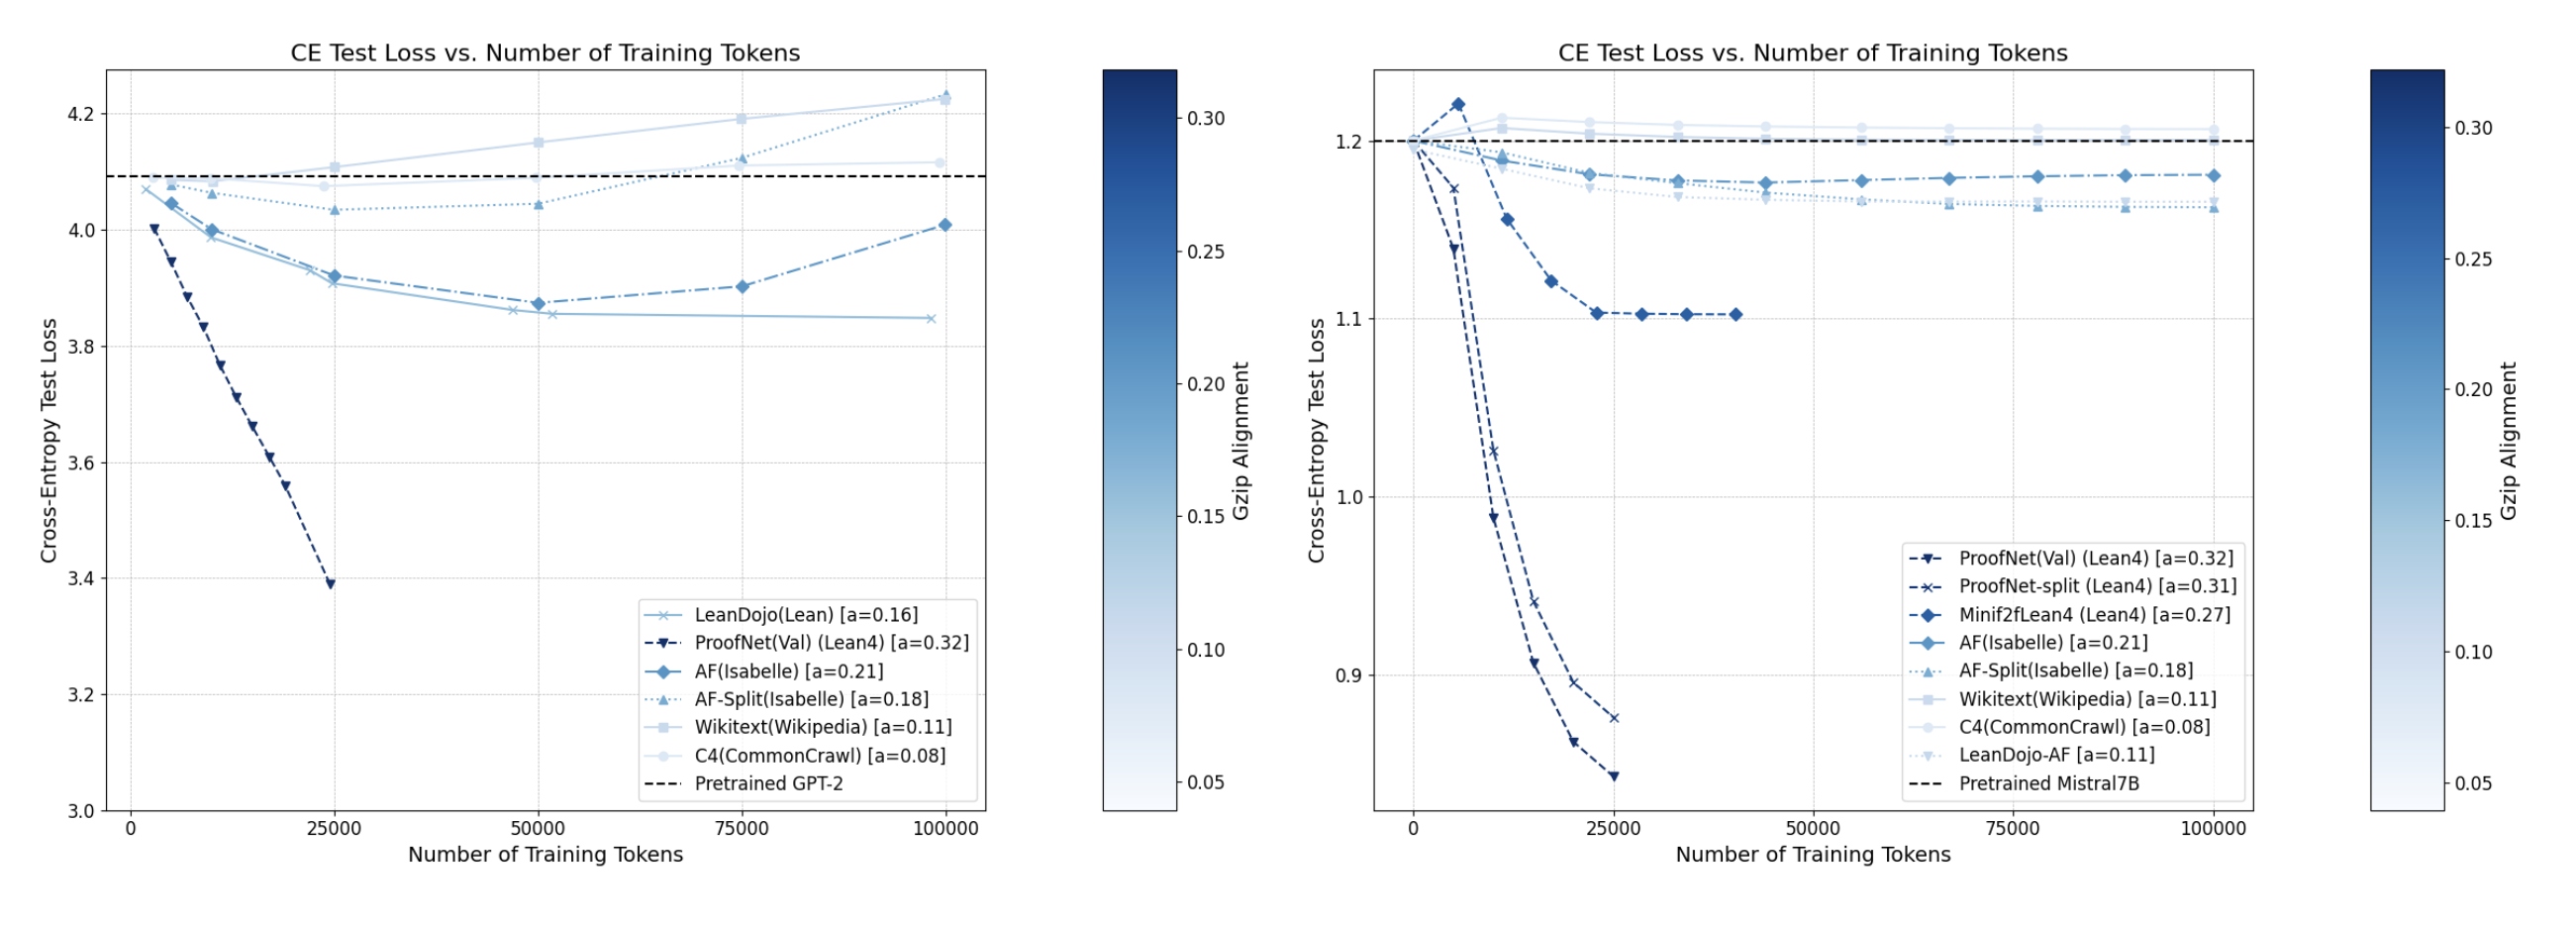
\includegraphics[width=1.0\textwidth]{./plots/more_alignment_lower_loss.png}}
  \caption{\textbf{Highly aligned data lowers cross-entropy loss more efficiently.} 
  The x-axis shows the number of training tokens, and the y-axis represents the cross-entropy (CE) test loss on the ProofNet test set. Different curves correspond to datasets filtered by different alignment scores, indicating their relevance to the target domain. The most aligned data reduce Test CE loss significantly faster than less aligned data. The left panel depicts results using GPT-2, and the right panel uses Mistral7B, demonstrating that using highly aligned data not only accelerates training but also achieves better model performance, validating the effectiveness of \texttt{ZIP-FIT} for data selection in fine-tuning.}
  \label{fig:more-alignment-lower-loss}
\end{figure*}
